\documentclass[a4paper]{article}     
\usepackage{amsfonts}
\usepackage{amsmath}
\usepackage{amssymb}
\usepackage{graphicx}

\begin{document}

\noindent \large Auteur: Ayoub Jaaouan \\
\noindent \large Studierichting: Informatica\\
\noindent \large Oefeningenreeks 3G nr. 2\\

\medskip

\normalsize

$f(x) = (x-2)^3 + 1$ \\

Nulpunten: \\

$f(x) = 0 \Rightarrow f(1) =  (1-2)^3 + 1 = 0 \Rightarrow x = 1$ \\

\bigskip

$f'(x) = 3(x-2)^2 $\\

Extrema: \\

$f'(x) = 0 \Rightarrow f(2) =  3(2-2)^2 = 0 \Rightarrow x = 2 $ \\

\bigskip

$f''(x) = 6(x-2) $\\

Buigpunten: \\

$f''(x) = 0 \Rightarrow f''(2) =  3(2-2)^2 = 0 \Rightarrow x = 2 $ \\

Tekenonderzoek.: \\

\begin{tabular}{l|lllll}
$x$ & $-\infty$ & $1$ & & $2$ & $-\infty$ \\ \cline{1-6}
$f(x)$ & $-$ & $0$ & $+$ & $+$ & $+$ \\
$f'(x)$ & $+$ & $+$ & $+$ & $0^{(2)}$ & $+$ \\
$f''(x)$ & $-$ & $-$ & $-$ & $0$ & $+$ \\ \cline{1-6}
$f(x)$ & $\frown$ & $0$ & $\frown$ & $B$ & $\smile$ \\
& $\nearrow$ & $0$ & $\nearrow$ & $(1)$ & $\nearrow$
\end{tabular}

\medskip

Raaklijn in punt $(1,0)$:\\

$y = 3(x-1)$ \\



\begin{figure}[h]
    \centering
    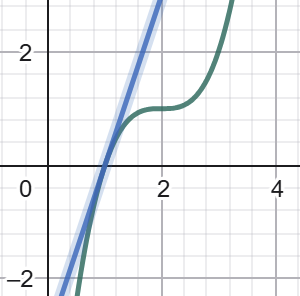
\includegraphics[width=0.5\textwidth]{3G-2-ayoub.jaaouan.INF.png}
\end{figure}

\begin{thebibliography}{999}
%\bibitem{a} Referentie
\end{thebibliography}
\end{document} 
